\chapter{Matter Has Far More Than Three States}

\begin{kaichang}
One summer, you order a box of ice cream online. Alongside the ice cream, the shipping carton contains several bulging bags holding chunks of ``ice'' that give off ``white smoke.'' You touch one through its bag---brrr, much colder than ice from the freezer. The instructions say: Dry ice. Do not touch directly with bare hands.

A few hours later, after finishing the ice cream, you remember those chunks and open a bag: empty. There is no water inside, the table is dry, and no residue lies in the trash. The ``ice'' has vanished without leaving even a drop of water.

Before reading on, guess the answers to three questions: Where did it go? What was that ``white smoke''? Why does ordinary ice melt into a puddle while this ice makes such a clean exit? By the end of this chapter, you should be able to answer all three with confidence.
\end{kaichang}

\section{The Three States We Can See}

Ice, water, and water vapor---the ``three states of matter'' you have known since childhood: solid, liquid, and gas. Set aside explanations and look only at the phenomena. What can you conclude?

A solid has its own shape and volume. An ice cube is a cube in a bowl and remains a cube on a plate. A liquid has volume but no shape of its own: water takes the shape of a bowl or bottle when poured into one. A gas has neither: after a soda bottle opens, the escaping gas spreads throughout the room. You cannot shape it or ``pile'' it in a corner.

Consider some other familiar scenes. A kettle emits a white cloud when water boils, but look closely: the cloud begins a short distance from the spout, not right at its opening. A mothball shrinks over several months without ever leaving a puddle of ``mothball water'' in the wardrobe. Wet clothes hung outdoors in winter first freeze stiff, yet become dry after a few days. Frost flowers appear on windows on bitterly cold mornings, though nobody has splashed water on the glass. A chilled drink can quickly collects droplets outside even though it is sealed. Where did the water come from? A large tank beside a filling station says ``liquefied petroleum gas''---how can gas be stored as a liquid? Matter changes state in all these scenes, but seemingly by different routes: some pass through liquid, others bypass it, and still others appear from thin air. To bring them together, we must zoom beyond what our eyes can see.

\section{Zooming In: What Are the Particles Doing?}

Chapter 1 explained that matter consists of tiny particles. Water consists of water molecules, and so do ice and water vapor. The particles themselves are identical in all three states. What changes is their \textbf{arrangement} and \textbf{motion}.

\begin{itemize}[itemsep=2pt]
\item \textbf{Solid}: particles sit tightly together, each ``held'' by its neighbors in a fixed position. They are not asleep: they vibrate constantly in place, like people in a room standing in assigned spots and jiggling their legs. Fixed positions give a solid its fixed shape.
\item \textbf{Liquid}: particles remain close together but are no longer locked in place. They squeeze and slide past one another, like passengers in a rush-hour subway car: pressed together, yet able to edge toward the door. Sliding allows flow and prevents a fixed shape; close packing keeps the volume essentially unchanged.
\item \textbf{Gas}: particles are suddenly much farther apart, racing about and colliding at random, like a handful of marbles scattered across a large playground. Wide spacing and freedom to roam give gases neither fixed shape nor fixed volume.
\end{itemize}

What is ``temperature'' in this picture? It is \textbf{a measure of how vigorously particles move}. In the same cup of water, higher temperature means molecules move faster and collide harder on average; lower temperature means slower motion. The ``hot'' feeling on your hand is the sensation of vast numbers of fast particles striking your skin and transferring energy.

And ``pressure''? Gas particles continually strike container walls. Billions upon billions of tiny impacts add up to pressure. Pump more air into a bicycle tire, and more frequent wall collisions make it firmer. Put a dented table-tennis ball in hot water: the gas inside warms, its particles strike harder, and the dent pops out. Macroscopic numbers such as temperature and pressure are collective expressions of particle motion.

\section{Six Names, One Rule}

\textbf{Translator safety note:} The fever example below is not treatment advice: do not use alcohol rubs to reduce fever, especially in children. Alcohol can cause poisoning through inhalation and skin absorption. See \href{https://www.poison.org/articles/rubbing-alcohol-only-looks-like-water}{Poison Control's alcohol warning}.

With our particle picture, we can give unified names to those apparently different routes. Three states allow six changes between pairs, and you have encountered them all:

\begin{itemize}[itemsep=2pt]
\item Solid $\rightarrow$ liquid: \textbf{melting} (ice becoming water); liquid $\rightarrow$ solid: \textbf{freezing} (water becoming ice).
\item Liquid $\rightarrow$ gas: \textbf{vaporization} (water becoming water vapor); gas $\rightarrow$ liquid: \textbf{liquefaction} (water vapor becoming water, also called condensation).
\item Solid $\rightarrow$ gas: \textbf{sublimation} (shrinking mothballs or drying frozen clothes); gas $\rightarrow$ solid: \textbf{deposition} (window frost, formed directly from indoor water vapor).
\end{itemize}

Behind the six names lies \textbf{one rule}: give particles energy, and they escape constraints toward greater freedom; when they release energy, they become more tightly bound. Melting, vaporization, and sublimation \textbf{absorb heat}; freezing, liquefaction, and deposition \textbf{release heat}. Freezing ice cubes makes a refrigerator consume electricity and emit heat because the energy released as water freezes must be carried away.

Two details deserve separate attention. First, vaporization takes two forms. \textbf{Evaporation} occurs at any temperature: some unusually fast molecules at the surface can always escape their neighbors' pull, so wet clothes slowly dry even in cloudy, rainy weather. \textbf{Boiling} requires a particular temperature and bubbles forming throughout the liquid. Evaporation carries away the fastest molecules, leaving slower average motion behind, so the remaining liquid \textbf{cools}. A fan cooling your sweaty body, doctors using diluted alcohol on skin to reduce a fever, and shivering in the wind after a swim all reflect the same rule: escaping molecules take energy with them.

Second, during melting or boiling, continued heating \textbf{no longer raises the temperature}. The added energy breaks constraints between particles instead of making them move faster. Chapters 27 and 28 will account for where that energy goes and why it must be spent, using energy and entropy. What holds particles together in the first place is the subject of Chapter 22.

\begin{shiyan}
\textbf{Observe Where the White Cloud Comes From} (An observation activity: a parent handles the hot water while you watch.)

Materials: a kettle or spouted saucepan, a flashlight (optional), and a cup of water at room temperature.

Procedure: (1) Ask a parent to boil the water. Once a white cloud emerges, turn off the heat but keep watching. (2) Examine the spout: does the cloud begin at the opening or a short distance away? (3) Shine the flashlight sideways through the cloud, then through the transparent region beside the spout where ``nothing seems to be there,'' and compare. (4) Hold a cup of cool water above the cloud, avoiding the steam because it can burn, and watch the cup's underside.

What to observe: Is anything present in the transparent region next to the spout? How far away does the white cloud begin? What happens beneath the cup?

Safety: Boiling water and steam can both cause serious burns. Never touch the spout, steam, or white cloud. Stay an arm's length away throughout.
\end{shiyan}

Careful observation reveals that the \textbf{transparent} region beside the spout contains the actual water vapor---a colorless, transparent gas invisible to your eyes. The white cloud consists of countless \textbf{tiny droplets} formed when vapor leaving the spout cools and condenses again: essentially a fine mist. The white cloud is therefore liquid, not gas. We will need this discovery when answering the opening questions.

\begin{qiaoliang}
How much does volume increase when liquid becomes gas? Let us calculate a real example. Take \ud{18}{mL} of water, roughly a tablespoon. Its mass is \ud{18}{g}, corresponding to $6.02\times 10^{23}$ water molecules (Chapter 5 introduces this enormous counting unit; for now, borrow the result). As water vapor at $100\,^{\circ}\mathrm{C}$ and atmospheric pressure, these molecules occupy about \ud{30}{L}---the size of a backpack. Volume has increased by about $30000\div 18\approx 1700$ times. The particles themselves have not grown: their average separation has increased by about $\sqrt[3]{1700}\approx 12$ times. Conversely, compressing gas into liquid can reduce its volume nearly a thousandfold, which is why a small canister of liquefied gas can fuel a stove for so long. When liquid vaporizes in a sealed container, it tries to expand over a thousandfold but cannot, so pressure rises sharply. Gas cylinders' warnings against direct sunlight and flames are no idle threats.
\end{qiaoliang}

\section{Symbols for Changes of State}

We can now introduce symbols. Chemistry indicates states with lowercase letters in parentheses: s for solid, l for liquid, g for gas, and aq for dissolved in water. Thus melting ice is written:

\[\chem{H_2O(s)} \rightarrow \chem{H_2O(l)}\]

Each substance has characteristic transition temperatures called its \textbf{melting point} and \textbf{boiling point}. These are among its fingerprints. Chapter 3's separation methods, including distillation and crystallization, exploit differences between such fingerprints. Here are several examples:

\begin{table}[htbp]
\centering
\begin{tabular}{lcc}
\toprule
Substance & Melting point ($^{\circ}\mathrm{C}$) & Boiling point ($^{\circ}\mathrm{C}$) \\
\midrule
Water & 0 & 100 \\
Alcohol (ethanol) & $-114$ & 78 \\
Nitrogen & $-210$ & $-196$ \\
Oxygen & $-218$ & $-183$ \\
Iron & 1538 & 2861 \\
\bottomrule
\end{tabular}
\end{table}

A glance explains many everyday arrangements. Winter thermometers in northern regions contain alcohol rather than water because water freezes at $0\,^{\circ}\mathrm{C}$, while alcohol remains liquid down to $-114\,^{\circ}\mathrm{C}$. Air cooled to around $-200\,^{\circ}\mathrm{C}$ becomes liquid; warming it gradually lets nitrogen and oxygen ``evaporate'' separately at their different boiling points. Industry produces oxygen by precisely this method.

Heat a cup of ice continuously and record its temperature over time, and you obtain a graph like this:

\begin{center}
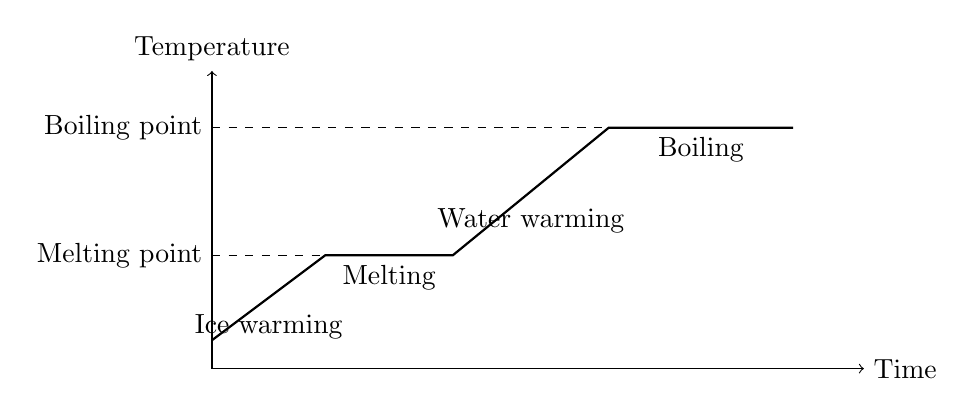
\begin{tikzpicture}[scale=0.9]
\draw[->] (0,0) -- (9.2,0) node[right] {Time};
\draw[->] (0,0) -- (0,4.2) node[above] {Temperature};
\draw[thick] (0,0.4) -- (1.6,1.6) -- (3.4,1.6) -- (5.6,3.4) -- (8.2,3.4);
\draw[dashed] (0,1.6) -- (3.4,1.6);
\draw[dashed] (0,3.4) -- (8.2,3.4);
\node[left] at (0,1.6) {Melting point};
\node[left] at (0,3.4) {Boiling point};
\node[below] at (0.8,0.9) {Ice warming};
\node[below] at (2.5,1.6) {Melting};
\node[below] at (4.5,2.4) {Water warming};
\node[below] at (6.9,3.4) {Boiling};
\end{tikzpicture}
\end{center}

The two plateaus represent melting and boiling: heat keeps entering, but temperature stays put. This is a schematic drawing; plateau widths and line slopes are not precise data. It clearly illustrates, however, how energy goes into breaking constraints before raising temperature.

\section{A Change of State Is Not a Chemical Change}

Return to Chapter 1's rule: what distinguishes physical from chemical change? Changes of state provide an excellent test.

However water shifts among ice, liquid, and vapor, its molecules remain \chem{H_2O}. The combination of two hydrogen atoms and one oxygen atom is neither broken apart nor rebuilt; only the looseness of arrangement and motion changes. A state change is therefore a \textbf{physical change}: the particles remain the same while their ``formation'' changes. The firm criterion is whether particles recombine, not whether something looks different. You have a way to test it: condense the white cloud back into water, and it is the same water as before, leaving no new substance when boiled away.

By contrast, using electricity to split water molecules into hydrogen and oxygen (Chapter 33) is chemical change: particles break apart and form new molecules that condensation or cooling cannot turn back into water. A state change alters the formation; a chemical change alters the team members.
\section{How ``Permanent Gases'' Were Overturned}

\begin{zhengju}
Today you know that any gas can become liquid if cooled sufficiently. In the early nineteenth century, nobody could guarantee that. Chemists readily liquefied chlorine and ammonia, but oxygen, nitrogen, and hydrogen stubbornly refused, however much pressure was applied. Textbooks therefore introduced ``permanent gases,'' supposedly incapable of liquefaction.

The breakthrough came through a sequence of accidents and one crucial insight. In 1823, Faraday heated a chlorine-containing compound in a sealed glass tube for another experiment and noticed an oily liquid condensing on the wall. He had inadvertently both compressed and cooled chlorine, liquefying it. Following the clue, he liquefied more than a dozen gases with ``pressure plus cooling,'' but oxygen, nitrogen, and hydrogen resisted.

The Irish physicist Andrews finally clarified the puzzle. In 1869, he systematically studied carbon dioxide at different temperatures and pressures and discovered something startling: above $31\,^{\circ}\mathrm{C}$, no amount of pressure liquefied it, and the boundary between gas and liquid disappeared altogether. He introduced the critical temperature: every gas has one, above which liquefaction is no longer possible. The ``permanent gases'' merely had critical temperatures below the reach of contemporary refrigeration. In 1877, oxygen and nitrogen were liquefied almost simultaneously; in 1908, the Dutch physicist Onnes liquefied even the most difficult gas, helium, reaching $-269\,^{\circ}\mathrm{C}$. ``Permanent gases'' disappeared from textbooks.

The lesson to take away is a way of thinking, not dates and names. Failure led beyond ``these gases are inherently special'' to a deeper question: was a necessary condition still missing? A concept repeatedly contradicted by experiment should make way for a better one. Andrews's disappearing liquid--gas boundary will return shortly.
\end{zhengju}

\section{Beyond the Three States}

``Solid, liquid, gas'' is a useful map, but it depicts the neighborhood of ordinary temperatures and pressures. Push either to extremes, or consider more complicated structures, and the boundaries blur. Every state below appears in daily life or the news.

\textbf{Plasma.} Heat gas above several thousand degrees, and increasingly violent collisions knock electrons out of atoms. The gas ceases to consist of intact neutral particles and becomes a ``soup'' of free electrons and charged ions: plasma, often called the fourth state of matter. Its charge makes it respond to electric and magnetic fields, its greatest difference from ordinary gas. Lightning channels, glowing neon tubes, and welding arcs are plasmas; the Sun and almost every star are enormous plasma balls. By mass, most observable matter in the universe occupies this state. The familiar ``three states'' are the cosmic minority.

\textbf{Liquid crystals.} Heating certain solids produces something odd: it flows like a liquid, but its molecules retain an orderly orientation instead of pointing every which way, giving it something of a crystal's character. This ``flowing order'' is a liquid crystal. A layer of liquid crystal lives in your phone screen: applying or removing voltage changes molecular orientation, altering light transmission and switching pixels on or off. Neither wholly solid nor wholly liquid, yet resembling both, it fits neither drawer of the three-state scheme.

\textbf{The glassy state.} Glass feels entirely solid, but at the particle level it lacks a crystal's orderly arrangement. Its disordered particles resemble a snapshot of a liquid, except they are frozen in place. This state, with liquidlike structure and solidlike behavior, is called the glassy state. Window glass, drinking glasses, glass fiber, refrigerator jelly, and hardened resin belong to this category. We will examine it again in Chapter 24 on crystals and new materials.

\begin{wuqu}
``Glass is actually an extremely slow-flowing liquid. Old European church windows are thicker at the bottom because the glass flowed downward over centuries.'' This widespread claim does not hold up. Flow requires particles to change position collectively, and at room temperature the time for glass particles to take a step is far longer than the universe's age. Centuries of flow would produce thickness changes below instrumental detection limits. Why, then, are old panes thicker below? Traditional flat glass was made from blown or spun disks with naturally uneven thickness, and installers usually placed the heavier edge downward. Indeed, old windows installed the other way, thicker at the top, also exist. The glassy state is a real category of solid, not a liquid too slow to see moving.
\end{wuqu}

\textbf{Supercritical fluids.} Remember Andrews's discovery: above a certain temperature and pressure---$31\,^{\circ}\mathrm{C}$ and about 73 atmospheres for carbon dioxide---the boundary between liquid and gas disappears. Matter in this region is neither liquid nor gas but a supercritical fluid combining properties of both: penetrating gaps like a gas and dissolving many substances like a liquid. This seemingly remote state may have helped fill your cup. Many instant coffees and teas are decaffeinated with supercritical carbon dioxide. It dissolves and removes caffeine while leaving most flavor compounds behind; releasing the pressure makes the carbon dioxide escape completely without residue.

``Far more than three states'' is therefore no figure of speech. The three-state model works very well for nearby temperatures and pressures, explaining everyday water, air, and metals. At excessive temperatures or pressures, or with special particle arrangements, we need a finer map. Scientific models cannot be judged simply as right or wrong; we ask how widely they work.

\section{Back to the Bag of Vanished ``Ice''}

We can now answer our three opening questions.

Dry ice is solid carbon dioxide at about $-78.5\,^{\circ}\mathrm{C}$. Its clean disappearance occurs because at ordinary atmospheric pressure carbon dioxide \textbf{has no liquid stage at all}: heating the solid makes it sublime directly into escaping gas. Why does carbon dioxide hurry while water follows the orderly ice--water--vapor route? The answer concerns each substance's territory on its state map; the challenge box gives a fuller explanation.

The ``white smoke'' is not carbon dioxide either. Like water vapor, carbon dioxide is a colorless, transparent gas invisible to your eyes. The cloud consists of countless tiny droplets formed when dry ice rapidly cools nearby air and condenses its water vapor, the same kind of mist as a kettle's white cloud. Stage fog and droplets on chilled drink cans follow the same principle: water has not leaked out of the can; atmospheric water vapor has surrendered to a cold surface.

The warning on the instructions now makes sense too: a temperature difference of around $79\,^{\circ}\mathrm{C}$ means contact with dry ice rapidly freezes water in skin tissue. Grabbing dry ice barehanded can cause injuries comparable to serious burns. Invisible dangers often deserve even greater respect than visible ones.

\section{From Freeze-Dried Coffee to Stars}

The rules of state changes have long worked quietly on industrial production lines, far beyond textbook vocabulary.

Food manufacturers use freeze-drying: freeze food thoroughly, then remove air to lower the pressure so its ice sublimes directly. Bypassing liquid prevents the cell structure from becoming water-damaged and best preserves nutrients and flavor. Freeze-dried coffee, fruit, and astronauts' meals depend on it, as do some heat-sensitive vaccines and medicines. Controlling seeds' moisture before storage likewise manages water's movements among solid, liquid, and gas.

Medicine and industry depend on liquid gases: hospital liquid oxygen, liquid nitrogen for welding, and liquid-nitrogen tanks preserving cells and tissues all ``concentrate'' gases hundreds or thousands of times for storage and transport. Plasma appears in fluorescent tubes, chip factories, and nuclear-fusion experiments. Scientists are trying to confine plasma hotter than a hundred million degrees with magnetic fields to imitate the Sun's energy production, one of humanity's ultimate energy gambles (Chapter 8 explains the nuclear reactions).

All these differences---why water freezes at $0\,^{\circ}\mathrm{C}$ and alcohol only at $-114\,^{\circ}\mathrm{C}$, why carbon dioxide skips liquid at atmospheric pressure, and why freezing water expands rather than contracts, allowing ice to float---ultimately point to the same hidden actor: \textbf{the invisible attraction between molecules}. It determines how tightly particles are held and how much energy releases them. Chapter 22 examines this invisible hand, while Chapter 23 puts water, that persistent eccentric, on trial.

\begin{tiaozhan}
(This box discusses phase diagrams; skipping it does not interrupt the main story.) Plot temperature horizontally and pressure vertically to create a state map called a phase diagram. Curves divide it into solid, liquid, and gas regions; each curve marks conditions where two states can coexist. One unique point, the \textbf{triple point}, permits all three simultaneously. Water's triple point is about $0.01\,^{\circ}\mathrm{C}$ and $0.006$ atmospheres, far below normal atmospheric pressure, so at normal pressure you can see the complete ice--water--vapor trilogy. Carbon dioxide's triple point is $-56.6\,^{\circ}\mathrm{C}$ and about $5.1$ atmospheres; liquid carbon dioxide occupies only the region \textbf{above} 5.1 atmospheres. Ordinary pressure never reaches its liquid territory, so heated dry ice crosses directly from solid to gas. This is the real reason it does not ``sweat.'' Carbon dioxide in extinguishers and cylinders is liquid precisely because their internal pressures far exceed this threshold.
\end{tiaozhan}

\section*{Try It Yourself}

\begin{sikaoti}
\item Draw particle diagrams for the solid, liquid, and gaseous states of one substance. Use dot spacing to show separation and short lines to show motion. Add a note: this representation helps us think; particles are not dots and do not really look like this.
\item Frozen clothes can slowly dry outdoors in winter. Explain with a particle picture how water molecules escape without the ice melting. What is this process called? Why do the clothes dry faster in sunny weather?
\item A pressure cooker cooks faster. Using the pressure--boiling-point relationship (higher pressure raises boiling point), explain what happens inside and why it makes food softer. Then consider why rice does not cook properly on a high plateau without a pressure cooker.
\item Estimate how much \ud{1}{L} of liquid nitrogen expands when fully vaporized at room temperature; its boiling point is $-196\,^{\circ}\mathrm{C}$. (Hint: follow the water-to-vapor calculation; an order-of-magnitude answer of several hundredfold is sufficient.) Explain why a liquid-nitrogen container must never be completely sealed.
\item Design an observation or experiment to convince a friend who insists a kettle's white cloud is water vapor that it is actually tiny droplets and that real vapor is invisible. Describe your procedure and expected observations.
\item A cup of water left on a table disappears after several days. Draw a material-flow diagram starting at the cup and tracing the molecules' destinations, labeling states and the conditions driving each step. What extra path appears if someone shuts the room's doors and windows tightly and puts out a bowl of ice?
\end{sikaoti}
